\documentclass[10pt, a4paper]{article}

\usepackage[spanish]{babel}
\usepackage{hyperref}

% fuente
\usepackage[sfdefault]{FiraSans}
\usepackage[T1]{fontenc}
\renewcommand*\oldstylenums[1]{{\firaoldstyle #1}}

% estilo parrafo
\usepackage[skip=10pt plus1pt, indent=0pt]{parskip}
\usepackage[skip=10pt plus1pt, indent=0pt]{parskip}
\usepackage{setspace}
\onehalfspacing
\hyphenpenalty 100
\hyphenation{Weekend}

\usepackage{graphicx} % Required for inserting images
\usepackage{svg}
\graphicspath{{Resources/}}
\usepackage{float}
\usepackage{amsmath}
\usepackage{subcaption}

\usepackage[style=numeric, sorting=none]{biblatex}
\addbibresource{bib.bib}


\title{TFG}
\author{Diego Sanz Fuertes}
\date{09 Agosto 2024}

\begin{document}
\maketitle
\titlepage
\tableofcontents
\newpage

\section{Introducción y objetivos}

La holografía es una técnica que permite capturar y reconstruir el campo de ondas completo de la luz. \cite{Goodman:2017} La holografía digital se utiliza hoy en día para varios propósitos, entre los que se encuentran los sistemas de pantallas tridimensionales (3D) \cite{Blinder:2019}. Las pantallas 3D holográficas permiten reproducir todas las señales de profundidad visuales naturales conocidas, como la oclusión, la acomodación del ojo, la convergencia y la estereopsis \cite{Blinder:2022}. Todas las señales de profundidad pueden observarse a simple vista en las pantallas holográficas, por lo que, en teoría, pueden reproducir una representación tridimensional fiel de cualquier escena sin restricciones en cuanto al contenido de la misma. Algunas de esas cualidades no se pueden conseguir por ejemplo con la representación 3D estéreo.

Los hologramas de un objeto se pueden obtener capturando el frente de ondas que proviene del objeto cuando se ilumina, proceso análogo a realizar una fotografía, fenómeno que también se puede simular generando el holograma mediante un computador, actividad análoga a la conocida generación de imágenes sintéticas por computador. Sin embargo, uno de los mayores desafíos de la generación de hologramas realistas por computador (CGH) es obtenerlos en tiempos computacionales aceptables \cite{Blinder:2019}.

En este trabajo de final de grado se implementan:
\begin{itemize}
    \item Un trazador de rayos estándar para generar imágenes sintéticas (2D) por computador el cuál simula el comportamiento de los rayos de luz basado en la física (Physically Based Ray Tracing o PBRT, en inglés).

    \item Además, se implementa un sistema de generación de hologramas (3D) por computador que hace uso de la técnica de modelado geométrico conocida como la nube de puntos y la técnica de trazado de rayos multiojo.

    \item Por último, con objeto de demostrar la validez de los resultados obtenidos, se visualizan los hologramas generados a partir de una escena virtual, tanto por simulación como en el laboratorio.

\end{itemize}

Dado que la exigencia computacional de este problema es muy alta y mucho mayor que las aplicaciones tradicionales de la computación gráfica, este proyecto propone una solución adecuada para abordar este problema que considera la arquitectura del software, los algoritmos y la alta paralelización del problema. Esta última, tanto en CPU como en GPU utilizando los lenguajes C++ y CUDA.

\section{Estado del arte}

La generación de imágenes sintéticas por computador (Computer-Generated Imagery o CGI, en inglés) es un campo de la computación gráfica bien estudiado que se utiliza en una gran variedad de áreas, como el diseño, la industria, el cine y los videojuegos. Consiste, en esencia, en capturar lo que vería un ojo al observar una escena virtual formada por objetos y fuentes de iluminación, a través de una pantalla pixelada obteniendo una imagen (tipo fotográfica) de dicha escena.

una escena virtual en un plano, para su posterior visualización.

Una de las técnicas más utilizadas en CGI es el trazado de rayos. En la literatura se pueden encontrar libros especializados que abordan tanto la teoría como la implementación con distintos niveles de profundidad. \cite{Shirley:2024} \cite{Pharr:2023}.

El trazado de rayos (o ray tracing, en inglés) es una técnica para simular la interacción de la luz con una escena para sintetizar escenas virtuales. Se considera una técnica computacionalmente costosa, por lo que es utilizada principalmente para renderización offline (no en tiempo real) con dispositivos computacionales habituales, o en tiempo real utilizando granjas de potentes procesadores y GPUs.

Un trazador de rayos completo ha de simular al menos los siguientes objetos y fenómenos \cite{Pharr:2023}: 

\begin{enumerate}
    \item Cámaras: El modelo de una cámara determina cómo y desde dónde la escena se observa, incluyendo como una imagen de la escena es recogida por un sensor.
    
    \item Intersecciones rayo-objeto: Es necesario conocer precisamente cuándo y dónde un rayo intersecta un objeto geométrico, además de determinar algunas propiedades del objeto en el punto de intersección.
    
    \item Fuentes de luz: El trazador de rayos ha de modelar la distribución de la luz en la escena.
    
    \item Visibilidad: Se debe poder conocer si una luz determinada deposita energía en un punto de una superficie.
    
    \item Dispersión de la luz en superficies: Cada objeto ha de proveer información sobre como la luz interactúa con la superficie del objeto.
    
    \item Transporte indirecto de luz: La luz puede llegar a la superficie después de rebotar o atravesar otras superficies.
    
    \item Propagación de rayos: Se necesita conocer el comportamiento de la luz mientras atraviesa un espacio, siendo su velocidad constante en el vacío.
    
\end{enumerate}

\underline{> Por hacer: ¿Esquema gráfico?}

Tal y como se ha dicho también es necesario generar hologramas. La generación de hologramas por computador (Computer-Generated Holography o CGH, en inglés) es una técnica que permite simular la captura del frente de ondas (3D) de una escena en un plano. 

Para entender el comportamiento de los CGH se debe tener presente la naturaleza de la luz. En esencia, una onda electromagnética se puede caracterizar en el espacio con su amplitud, su fase y su longitud de onda. El formalismo matemático general viene dado por las ecuaciones de Maxwell \cite{Goodman:2017} y su solución general es inabordable con la capacidad de cálculo actual.

Por este motivo, se buscan simplificaciones que permitan modelar adecuadamente el comportamiento de ondas electromagnéticas. En el caso que nos ocupa, supondremos siempre ondas monocromáticas, en el rango óptico escalar y en medios isótropos. En estas condiciones, podemos obviar la parte temporal de la onda y centrar los cálculos en la propagación espacial de la misma.

Supongamos que en un punto de espacio llegan ondas electromagnéticas de N fuentes puntuales de luz. El valor que llega se pueda calcular según la \autoref{eq:amplitud-fase} \cite{Goodman:2017}.

\begin{equation}
H(x,y) = \sum\limits_{j=1}^N a_j\exp\Big(\frac{\pi i}{\lambda z_j}\big[(x-x_j)^2 + (y-y_j)^2 \big]\Big)
\label{eq:amplitud-fase}
\end{equation}

Donde H es el valor de la onda en el punto $x,y$, a es la amplitud de cada una de las fuentes puntuales que llegan a ($x,y$), $\lambda$ es la longitud de onda y ($x_{j},y_{j},z_{j}$) son las coordenadas de cada fuente puntual. Siendo $a_j$ la amplitud y el valor complejo del exponencial la fase.

El cálculo de un CGH es, en esencia, el cálculo de la onda electromagnética resultante que llega a cada uno de los píxeles del sensor.

En el estudio \cite{Blinder:2022} se ofrece una visión general del estado del arte en CGH, una clasificación de los algoritmos y diferentes técnicas de aceleración.

Entre los algoritmos clasificados se encuentran los dos que se van a utilizar en este trabajo:

\begin{itemize}
\item Nube de puntos: Esta técnica consiste en la suma de todas las funciones de dispersión de puntos (PSFs), en el plano del holograma, que emanan de una colección de puntos luminosos. Se entiende la PSF como la función que describe respuesta de un sistema de imagen a un objeto o fuente puntual. Se puede observar en la figura \autoref{fig:nube-de-puntos} la función de dispersión de un punto de la escena evaluada en un plano. Las principales limitaciones de esta técnica son (1) la falta de soporte de efectos básicos como la oclusión y el sombreado; y (2) el alto coste computacional, aunque el algoritmo es altamente paralelizable \cite{Blinder:2021}

\begin{figure}[H]
    \centering 
    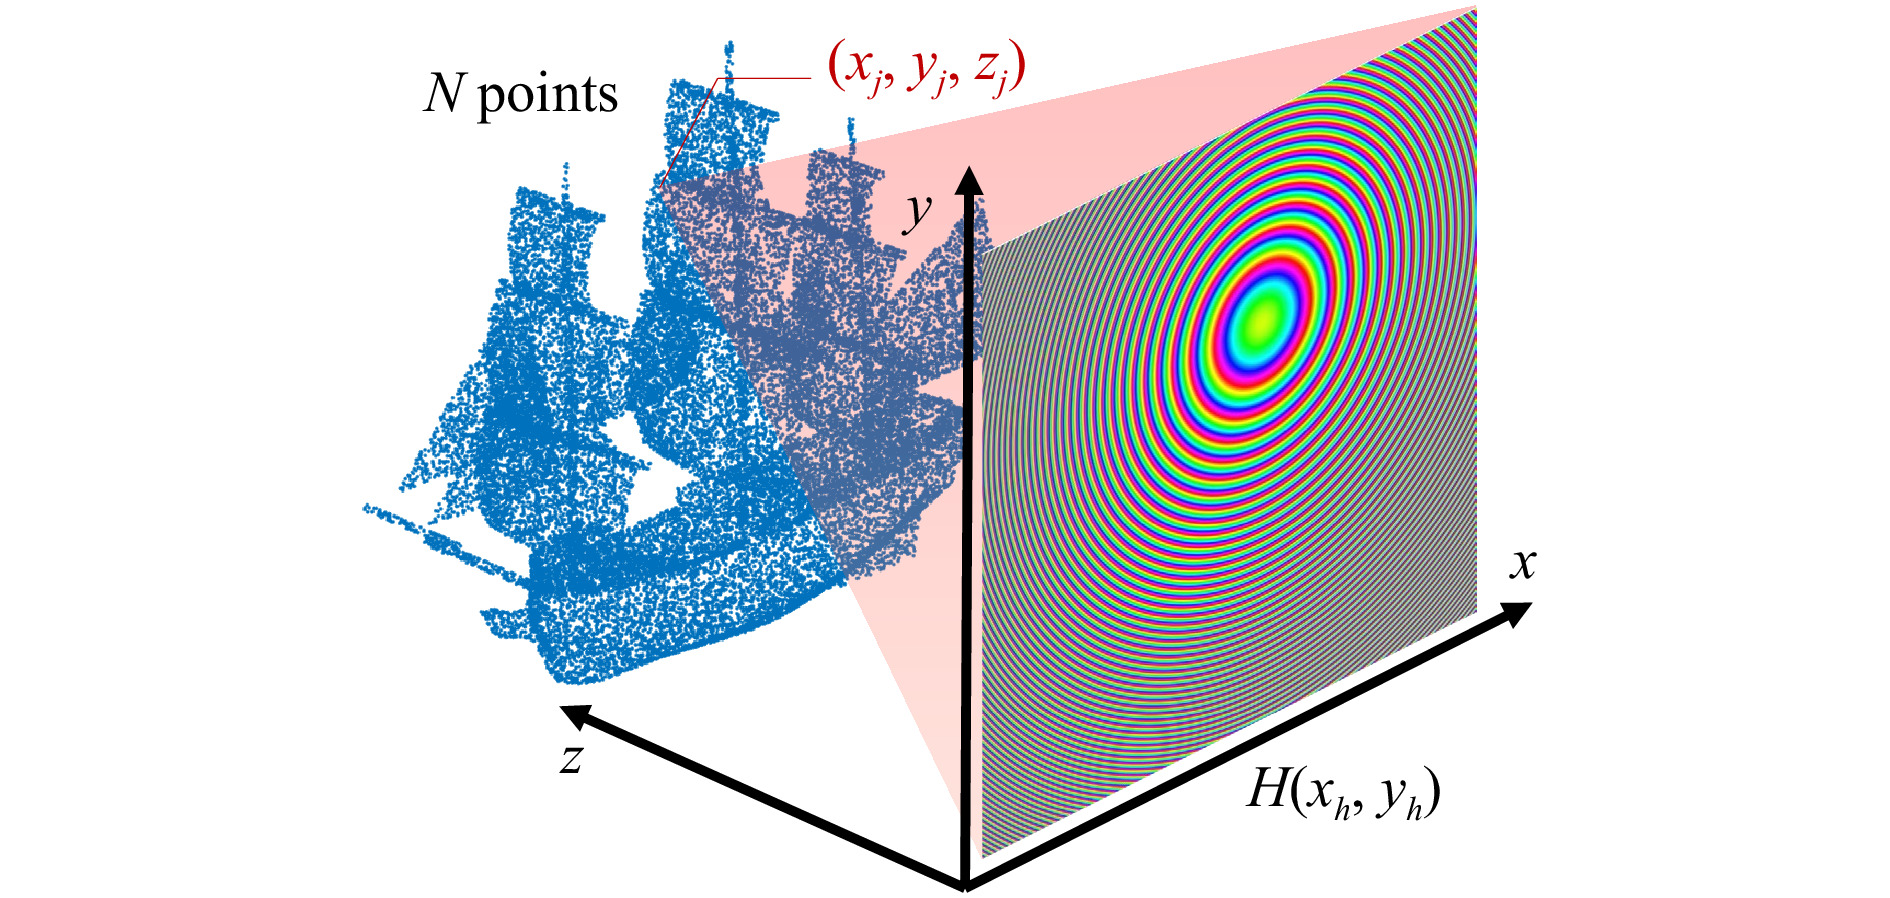
\includegraphics[width=0.75\textwidth]{tecnica_nube_puntos}
    \caption{Diagrama del algoritmo de la nube de puntos. Fuente: \textcite{Blinder:2022}.}
    \label{fig:nube-de-puntos}
\end{figure}

\item Trazado de rayos: Es una técnica para modelar el transporte de la luz basada en el seguimiento de rayos de luz individuales que rebotan en la escena e interactúan con materiales, calculando con precisión la cantidad de luz alcanzando cada píxel de la cámara virtual. Esta técnica puede aprovecharse en CGH para modelar también el transporte de la luz. Sin embargo, no puede utilizarse directamente, ya que la holografía se basa fundamentalmente en ondas, lo que difiere sustancialmente de los modelos basados en rayos. Uno de los principales problemas es la necesidad de obtener un continuo de puntos de vista y otro problema es la falta de coherencia de fase de la luz. Estos dos problemas hacen que los métodos basados en el trazado de rayos han de ser adaptados o combinados con otros algoritmos para ser utilizados efectivamente \cite{Blinder:2022}.
\end{itemize}

En \cite{Blinder:2021} se propone un método híbrido que toma los mejores aspectos de los métodos de nube de puntos y del trazado de rayos. En vez de calcular directamente el campo de luz en el plano del holograma, se calcula la intensidad en cada punto de la nube de puntos de la escena mediante trazado de rayos, y se calcula la PSF con esa intensidad. De este modo se consiguen efectos de iluminación realistas, sin comprometer la coherencia de la fase, lo que da lugar a vistas continuas y señales de profundidad precisas.

La naturaleza del algoritmo de trazado de rayos permite que pueda ser acelerado mediante paralelización, ya que los rayos son independientes unos de los otros \cite{Chalmers:2002}. En \cite{Blinder:2021} se paraleliza en GPUs mediante CUDA y OptiX.

Como se ha mencionado anteriormente, el cálculo de propagación de ondas electromagnéticas utilizando la técnica de nube de puntos tiene un coste computacional elevado. Existe la posibilidad de disminuir drásticamente los tiempos de cálculo cuando se pretende conocer la propagación de ondas entre dos planos que son paralelos entre sí. En estas condiciones se pueden utilizar los algoritmos de convolución y de transformada de Fourier, bien descritos en la literatura \cite{Goodman:2017}. Se trata de conocer los valores de la onda $U$ en el plano $(x,y)$ a partir de los valores conocidos de la misma en el plano $(\xi, \eta)$ según descrito en la \autoref{eq:propagacion}. 

\begin{equation}
U(x, y)=\frac{e^{i k z}}{i \lambda z} \exp \left(\frac{i k}{2 z}\left(x^2+y^2\right)\right) \iint_{-\infty}^{\infty}\left\{U(\xi, \eta) e^{\frac{i k}{2 z}\left(\xi^2+\eta^2\right)}\right\} e^{-i \frac{2 \pi}{\lambda z}(x \xi+y \eta)} d \xi d \eta
\label{eq:propagacion}
\end{equation}

\section{Proceso de síntesis de escenas virtuales en 3D mediante hologramas digitales}

La implementación del algoritmo desarrollado se ha realizado mediante el uso de los lenguajes C++ y CUDA para la definición de la escena virtual y la generación de hologramas digitales, y Python para la reconstrucción de la escena. Las librerías utilizadas se enumeran en el anexo Repositorios.

Todas las figuras mostradas son de elaboración propia, tanto los diagramas como los renderizados, a no ser que se indique lo contrario.

\subsection{Definición de la escena virtual}

El primer paso para la síntesis de escenas virtuales consiste en definir la escena que se desea producir. Veamos el siguiente ejemplo (\autoref{fig:render-ejemplo}):

\begin{figure}[H]
    \centering 
    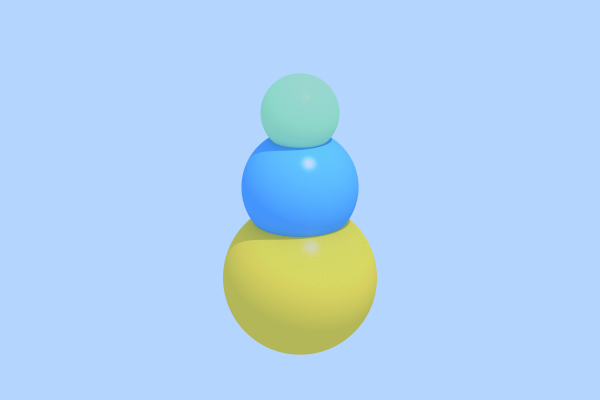
\includegraphics[width=0.75\textwidth]{00_example}
    \caption{Render}
    \label{fig:render-ejemplo}
\end{figure}

Esta escena está definida por el color del cielo, la posición, el tamaño y el material de las tres esferas, y la posición y color de una fuente de luz puntual. En pseudocódigo se podría definir de la siguiente manera (números en milímetros):

\begin{verbatim}
sky_color: light_blue;

Sphere(center: (0, 1.4, -1), 
       radius: 0.2, 
       material: Lambertian(albedo: light_green);
Sphere(center: (0, 1, -1), 
       radius: 0.3, 
       material: Lambertian(albedo: light_blue));
Sphere(center: (0, 0.5, -1), 
       radius: 0.4, material: 
       Lambertian(albedo: yellow);
       
PointLight(position: (3, 11, 3), color: white);
\end{verbatim}

\subsubsection{Geometría}

La geometría de la escena se definirá mediante primitivas definidas matemáticamente. Estas primitivas son: triángulos, definidos mediante la posición espacial de sus vértices; y esferas, definidas mediante su radio y la posición espacial de su centro. 

Utilizando la primitiva del triángulo se pueden representar mallas, definidas por una lista de triángulos. El soporte de mallas resulta muy útil ya que la mayoría de modelos 3D se encuentra en este formato. 

\subsubsection{Textura}

Una vez definida la geometría de la escena, es necesario aplicar texturas a las primitivas. Las texturas que se han utilizado no siguen el significado tradicional de imágenes bidimensionales mapeadas sobre la superficie de la geometría, si no que se emplean distintos tipos de materiales, detallados a continuación:

\begin{enumerate}
    
\item Material difuso (lambertiano): Este material dispersa la luz siguiendo una distribución independiente al ángulo de incidencia y proporcional al coseno del ángulo formado entre la normal de la superficie y la dirección de dispersión. Esta distribución viene dada por la ley del coseno de Lambert. El color y la intensidad de la luz se ven modificados por el color (o albedo) del material. Este material podría describirse como mate. En la \autoref{fig:render-difuso} se puede apreciar el comportamiento del material difuso y en la \autoref{fig:diagrama-difuso} se muestra un diagrama de la reflexión difusa lambertiana.

\begin{figure}[H]
    \centering 
    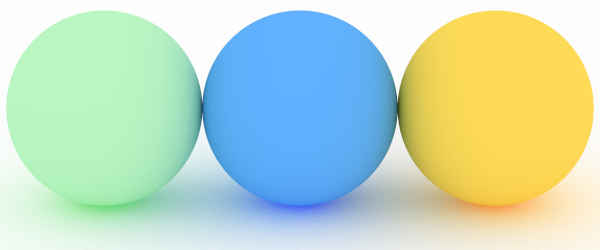
\includegraphics[width=0.75\textwidth]{02_crop}
    \caption{Render de tres esferas de diferentes colores sobre una superficie blanca. Materiales difusos.}
    \label{fig:render-difuso}
\end{figure}

\begin{figure}[H]
    \centering 
    \includesvg[width=0.75\textwidth]{lambertian}
    \caption{Diagrama de la dispersión de un material difuso lambertiano. En negro, el rayo de luz incidente, en rojo, la distribución de la dirección e intensidad de la dispersión.}
    \label{fig:diagrama-difuso}
\end{figure}

\item Material metálico: Al contrario que el material difuso, el material metálico refleja la luz en el mismo ángulo en dirección opuesta respecto al ángulo de incidencia (véase \autoref{fig:render-metalico}). Este efecto produce un reflejo de la misma manera que un espejo. Este material también cuenta con un parámetro que controla la borrosidad (o fuzziness, en inglés) del reflejo. En la \autoref{fig:diagrama-metalico} se puede observar el efecto espejo del material junto a el parámetro de borrosidad.

\begin{figure}[H]
    \centering 
    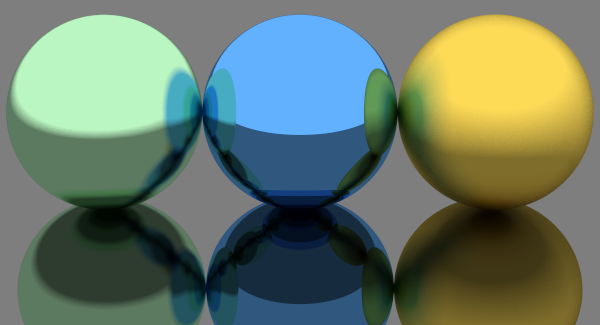
\includegraphics[width=0.75\textwidth]{03_crop}
    \caption{Render de tres esferas de diferentes colores sobre una superficie gris. Materiales metálicos con distinta borrosidad: 0.1 (izquierda), 0 (centro y superficie) y 0.5 (derecha).}
    \label{fig:render-metalico}
\end{figure}

\begin{figure}[H]
    \centering 
    \includesvg[width=0.75\textwidth]{metalic}
    \caption{Diagrama de la reflexión de un material metálico sin borrosidad. Rayo de incidencia en negro, rayo reflejado en rojo y vector normal a la superficie en azul.}
    \label{fig:diagrama-metalico}
\end{figure}

\item Material dieléctrico: Este material representa materiales transparentes como agua y cristal. Cuando la luz incide sobre el material, se divide en luz reflejada (como el material metálico) y en luz refractada. La reflectividad se describe según las ecuaciones de Fresnel y la refracción según la ley de Snell como se puede observar en la \autoref{fig:diagrama-dielectrico}. Este material también cuenta con un parámetro que controla el índice de refracción. En la \autoref{fig:render-dielectrico} se puede apreciar el efecto de distintos índices de refracción. También se puede observar la luz refractada en la bola de la derecha debido a un índice de refracción elevado. Cabe destacar que las bolas de materiales dieléctricos no tienen sombra, se puede comprobar que ese es el caso observando una bola de cristal en un día nublado.
\end{enumerate}


\begin{figure}[H]
    \centering 
    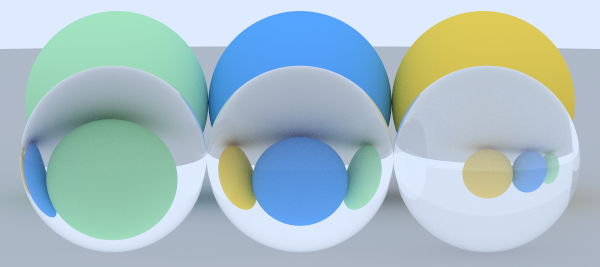
\includegraphics[width=0.75\textwidth]{04_crop}
    \caption{Render de tres bolas con un material dieléctrico y tres esferas de distintos colores, sobre una superficie gris. Los índices de refracción de las tres bolas son: 1.3 (agua, izquierda), 1.5 (cristal, centro) y 2.4 (diamante, derecha).}
    \label{fig:render-dielectrico}
\end{figure}

\begin{figure}[H]
    \centering
    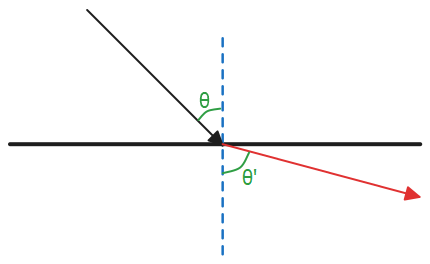
\includegraphics[width=0.75\textwidth]{dielectric}
    \caption{Diagrama de la refracción y reflexión de un rayo de luz al atravesar la superficie de un material dieléctrico. Rayo de incidencia en negro, rayo refractado en rojo y rayo reflejado discontinuo.}
    \label{fig:diagrama-dielectrico}
\end{figure}

También existen otras formas más completas de definir materiales como las descritas en los modelos de Disney \cite{Burley:2012} o OpenPBR \cite{Academy-Software-Foundation:2024}.

Finalmente, en la \autoref{fig:render-materiales} se puede observar un render de una escena la cual contiene todos los materiales.

\begin{figure}[H]
    \centering 
    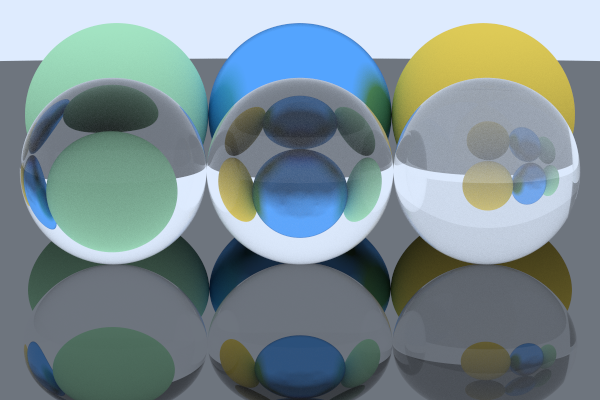
\includegraphics[width=0.75\textwidth]{01_materials}
    \caption{Render demostrando los distintos materiales. Basado en el render de la \autoref{fig:diagrama-dielectrico} (superficie y esfera azul metálicas con borrosidad 0 y 0.3 respectivamente).}
    \label{fig:render-materiales}
\end{figure}

\subsubsection{Iluminación}

La última sección de la definición de la escena virtual es la iluminación. La iluminación que se utiliza se puede dividir en dos tipos de fuente: el cielo y fuentes puntuales de luz.

El cielo ilumina de manera uniforme la escena mientras que las fuentes de luz puntuales siguen el modelo de reflexión de Blinn-Phong \cite{Blinn:1977}, que describe la forma en la que una superficie refleja la luz como una combinación de la iluminación difusa y la iluminación especular. No se incluye el término ambiental del modelo ya que se utiliza el cielo. En la \autoref{fig:iluminacion} se pueden observar los componentes por separado.

\begin{figure}[H]
    \centering 
    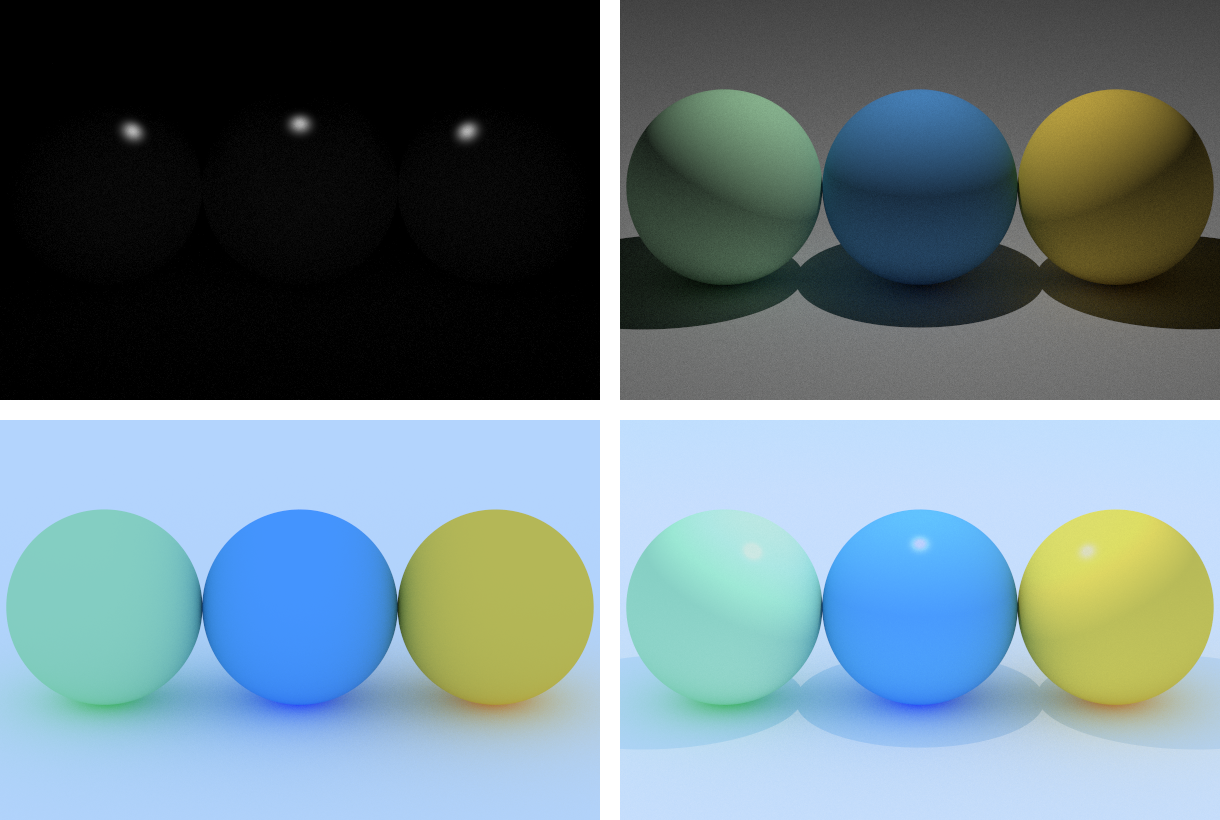
\includegraphics[width=0.75\textwidth]{05_agg}
    \caption{Render de tres esferas con iluminación puntual e iluminación ambiente, separado en sus componentes: Especular (superior izquierda), difuso por punto de luz (superior derecha), difuso por iluminación ambiente (inferior izquierda) y componentes agregados (inferior derecha).}
    \label{fig:iluminacion}
\end{figure}

En la \autoref{fig:holograma-cgi} se muestra la escena que se utilizará como referencia para la generación de hologramas. Se encuentra iluminada por una fuente de luz puntual de color rojo, ya que es la longitud de onda con la que se trabaja en el laboratorio. La definición en pseudocódigo es la siguiente (en mm):

\begin{verbatim}

Sphere(center: (-0.8, 0.25, -12), 
       radius: 3,
       material: Lambertian(albedo: magenta));
Sphere(center: (1, -0.25, 0),
       radius: 2,
       material: Lambertian(albedo: magenta));
Sphere(center: (2, 2, 5), 
       radius: 0.5,
       material: Lambertian(albedo: magenta));

Camera(look_from: (0, 0, 200),
       look_at: (0, 0, 0),
       diffuse_intensity: 100%,
       specular_intensity: 0%,
       sky_intensity: 0%);

PointLight(position: (5000, 5000, 10000), color: red);

\end{verbatim}

\begin{figure}[H]
    \centering 
    \includegraphics[width=0.75\textwidth]{07_holo_cgi}
    \caption{Render de tres esferas que proyectan sombras entre ellas, iluminadas por una fuente de luz puntual de color rojo.}
    \label{fig:holograma-cgi}
\end{figure}

\subsection{Generación de imágenes por computador (CGI)}

En este apartado se detalla el algoritmo de trazado de rayos utilizado para generar imágenes y hologramas, explicando cómo se simulan los rayos de luz desde la fuente hasta el detector.

En este trabajo concretamente se utiliza el algoritmo de trazado de caminos (o path tracing, en inglés), el cual simula más efectos que el trazado de rayos convencional gracias al uso de simulaciones de Monte Carlo (utilizando muestreo aleatorio).

En la \autoref{fig:diagrama-rebotes} se puede observar el posible comportamiento de un rayo en una escena sencilla.

\begin{figure}[H]
    \centering 
    \includesvg[width=0.75\textwidth]{bounces}

    \caption{Diagrama que muestra uno de los posibles caminos de un rayo de luz en una escena sencilla.}
    \label{fig:diagrama-rebotes}
\end{figure}

Como se ha mencionado anteriormente, el algoritmo se ha implementado en el lenguaje de programación C++ debido a su alto rendimiento, control sobre conceptos de bajo nivel (como gestión de la memoria) y compatibilidad con CUDA para acelerar mediante GPUs. La implementación inicial se ha basado en el libro Ray Tracing in One Weekend \cite{Shirley:2024} (el resultado de la escena final se puede observar en la \autoref{fig:render-final}) y se han añadido más funcionalidades no incluidas en el libro.

El primer componente del trazador de rayos es la cámara, encargada de lanzar los rayos ya que la propagación desde la fuente de luz hasta la cámara es equivalente a la propagación desde la cámara hasta la fuente de luz. La cámara se basa en una cámara estenopeica (o cámara oscura) sin lente, aunque también es capaz de simular una lente para obtener el efecto de profundidad de campo.

\begin{figure}[H]
    \centering 
    \includesvg[width=0.75\textwidth]{camera}
    \caption{Diagrama del modelo de cámara utilizado, basado en una cámara estenopeica.}
    \label{fig:diagrama-camara}
\end{figure}

La cámara se define mediante su centro y su viewport (véase \autoref{fig:diagrama-camara}). El centro de la cámara es el punto (o el centro del disco en el caso de simular una lente) desde el cuál se originan los rayos. El viewport es un rectángulo bidimensional discretizado en píxeles utilizado para proyectar la escena. Cada píxel del viewport se corresponde con el de la imagen de salida por lo que se podría hacer un símil con el sensor de la cámara. Cada píxel indica la dirección de un rayo (véase \autoref{fig:diagrama-camara-2}) y una vez trazado el rayo se almacena el color resultante en la imagen de salida. Se puede obtener mayor calidad perceptual al elegir un punto aleatorio dentro del píxel en vez de su centro y se puede reducir el aliasing y aumentar la calidad al mediar el resultado de varias muestras del píxel (véase \autoref{fig:diagrama-muestreo}).

\begin{figure}[H]
    \centering 
    \includesvg[width=0.75\textwidth]{camera_rays}
    \caption{Diagrama del funcionamiento de la cámara en el algoritmo de trazado de rayos. Los rayos comienzan en el centro de la cámara en dirección al centro de cada píxel del viewport.}
    \label{fig:diagrama-camara-2}
\end{figure}

\begin{figure}[H]
    \centering 
    \includesvg[width=0.75\textwidth]{camera_samples}
    \caption{Diagrama del muestreo aleatorio realizado a nivel de píxel. Utilizado para reducir el aliasing y aumentar la calidad.}
    \label{fig:diagrama-muestreo}
\end{figure}

Una vez lanzado el rayo se comprueba si intersecta con algún objeto de la escena iterando sobre ellos y se selecciona el objeto intersectado más cercano. De la intersección se obtiene el punto, la distancia respecto al origen del rayo, la normal de la superficie y el material del objeto. Con esta información, para la iluminación ambiente, se puede calcular la atenuación y la dirección del rayo dispersado dependiendo del material. Este proceso se repite hasta que el rayo dispersado no intersecta ningún objeto (o escapa de la escena) y se atenúa con el color del cielo o, si alcanza el número máximo de rebotes definido por el trazador de rayos, la atenuación sería total. Y para la iluminación puntual, siguiendo la misma ruta del rayo de la iluminación ambiente, se comprueba si el punto es visible para la fuente de luz trazando un rayo nuevo y, si lo es, se calcula la iluminación especular y la iluminación difusa, esta última en el caso de que el material sea difuso. 

También se ha creado una interfaz de usuario para agilizar el proceso de desarrollo que permite modificar en tiempo de ejecución distintos parámetros, como los ajustes de renderizado, la posición y orientación de la cámara, la iluminación y los materiales de los objetos (\autoref{fig:gui}).

\begin{figure}[H]
    \centering 
    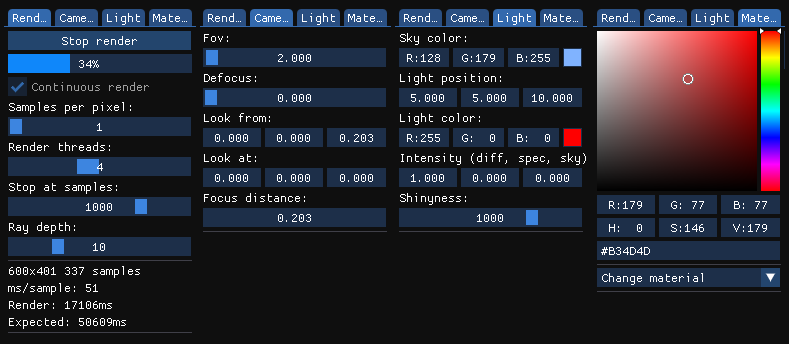
\includegraphics[width=0.75\textwidth]{gui_parameters}
    \caption{Parámetros de la interfaz de usuario.}
    \label{fig:gui}
\end{figure}

\begin{figure}[H]
    \centering 
    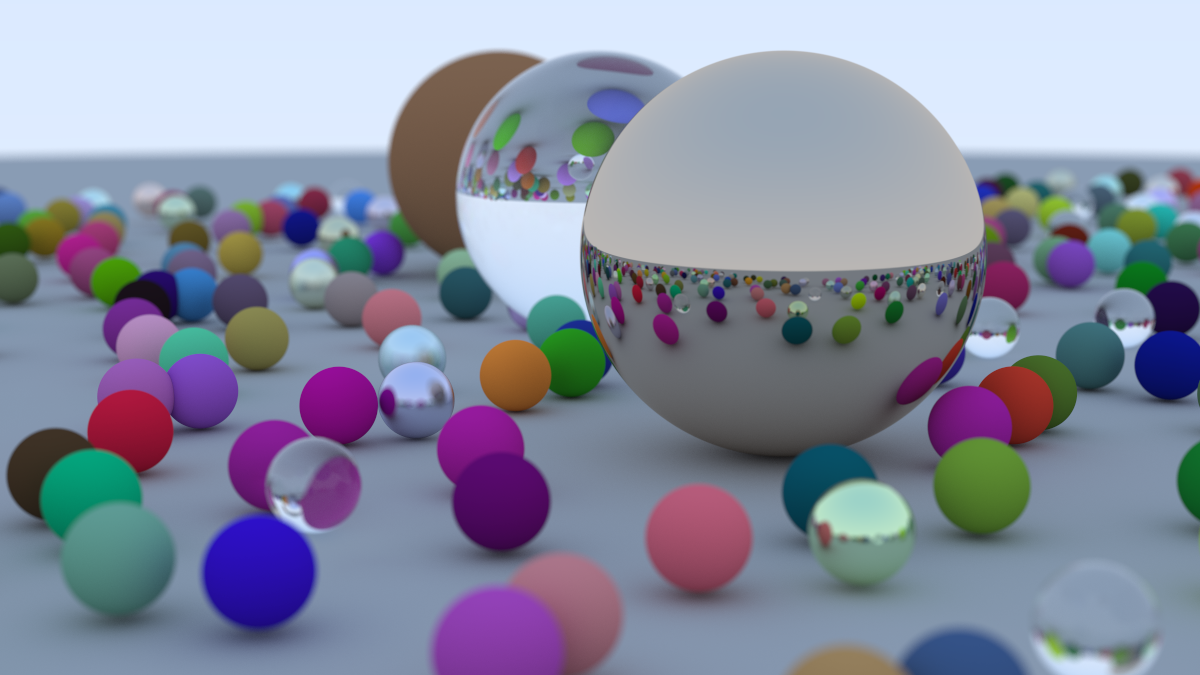
\includegraphics[width=0.75\textwidth]{06_end_book_1}
    \caption{Render de la escena final descrita en el libro Raytracing in one Weekend \cite{Shirley:2024}. Elaboración propia.}
    \label{fig:render-final}
\end{figure}

\subsection{Generación de hologramas por computador (CGH)}

Una vez implementado el trazador de rayos para la generación de imágenes, se ha modificado para generar hologramas. Las principales modificaciones realizadas han sido el proceso de lanzar rayos y el cambio del cálculo del color del rayo al cálculo de la amplitud y fase (mediante la \autoref{eq:amplitud-fase}).

Para obtener la amplitud y la fase de cada rayo que llega a cada píxel del holograma se ha de calcular respecto a cada punto de la escena a muestrear, siendo los mismos puntos para cada píxel. Para determinar los puntos de la escena se ha utilizado la técnica de la nube de puntos, según la cual se construye una lista de puntos en las superficies de los objetos de la escena (véase \autoref{fig:diagrama-camara-slm}). En la implementación, la nube de puntos se calcula una sola vez y se puede generar mediante rayos perpendiculares al viewport o mediante rayos con el origen en el centro del sensor y dirección a cada píxel del viewport.

\begin{figure}[H]
    \centering 
    \includesvg[width=0.75\textwidth]{slm}
    \caption{Diagrama del modelo de cámara utilizado para generar hologramas. Arriba, creación de la nube de puntos; abajo, desde cada píxel del sensor se lanza un rayo en dirección a cada punto de la nube de puntos.}
    \label{fig:diagrama-camara-slm}
\end{figure}

La amplitud y la fase se calcula según lo descrito en la \autoref{eq:amplitud-fase}.

Una vez generado el holograma es almacenado en dos archivos, uno contiene la amplitud y el otro la fase. Como el holograma almacenado es bidimensional, se puede almacenar en formatos de imagen como PNG. Estos archivos serán los utilizados posteriormente para la reconstrucción de la escena. La representación visual de los archivos se puede observar en la \autoref{fig:amplitud-y-fase}.

\begin{figure}[H]
\centering
    \begin{subfigure}{1\textwidth}
        \includegraphics[width=1\textwidth]{phase}
        \caption{Amplitud}
        \label{fig:amplitud-y-fase-a}
    \end{subfigure}
    \begin{subfigure}{1\textwidth}
        \includegraphics[width=1\textwidth]{amplitude}
        \caption{Fase}
        \label{fig:amplitud-y-fase-b}
    \end{subfigure}
    \caption{Representación gráfica de la amplitud y fase de un holograma almacenado, generado a partir de la escena descrita en la \autoref{fig:holograma-cgi}.}
    \label{fig:amplitud-y-fase}
\end{figure}

\subsection{Reconstrucción de la escena}

Para recuperar la escena se debe realizar el proceso inverso al definido en la sección anterior; esto es, se debe propagar una onda electromagnética desde el plano del CGH hasta los diferentes planos que constituyen la escena.

Se han utilizado dos procesos para la reconstrucción de la escena: simulación mediante la propagación de ondas electromagnéticas entre dos planos y propagación en el laboratorio mediante un modulador espacial de luz (SLM), modelo PLUTO-2.1 LCOS, y un láser con longitud de onda de 632.8nm.

La simulación es computacionalmente mucho menos exigente que la generación, ya que podemos utilizar los algoritmos de convolución y de transformada de Fourier para reducir considerablemente el tiempo de cómputo para simular el comportamiento de la luz a su paso por el CGH.

La reconstrucción puede hacer uso de la fase almacenada en el holograma, de la amplitud o de ambas. Ya que el SLM del que se dispone en el laboratorio solamente es capaz de modular la fase, ambas reconstrucciones se han llevado a cabo utilizando solamente la información de la fase con el fin de obtener resultados comparables.

El resultado de reconstruir la escena previamente definida (\autoref{fig:holograma-cgi} y almacenada (\autoref{fig:amplitud-y-fase} se puede observar en la \autoref{fig:reconstruccion}. Ambas reconstrucciones están enfocadas en la esfera mediana ($z=200$). En la \autoref{fig:reconstruccion-figura} se ha simulado la propagación en distintos valores de $z$ y se puede apreciar el desenfoque de las distintas esferas.

\begin{figure}[H]
    \centering
    \begin{subfigure}{1\textwidth}
        \centering
        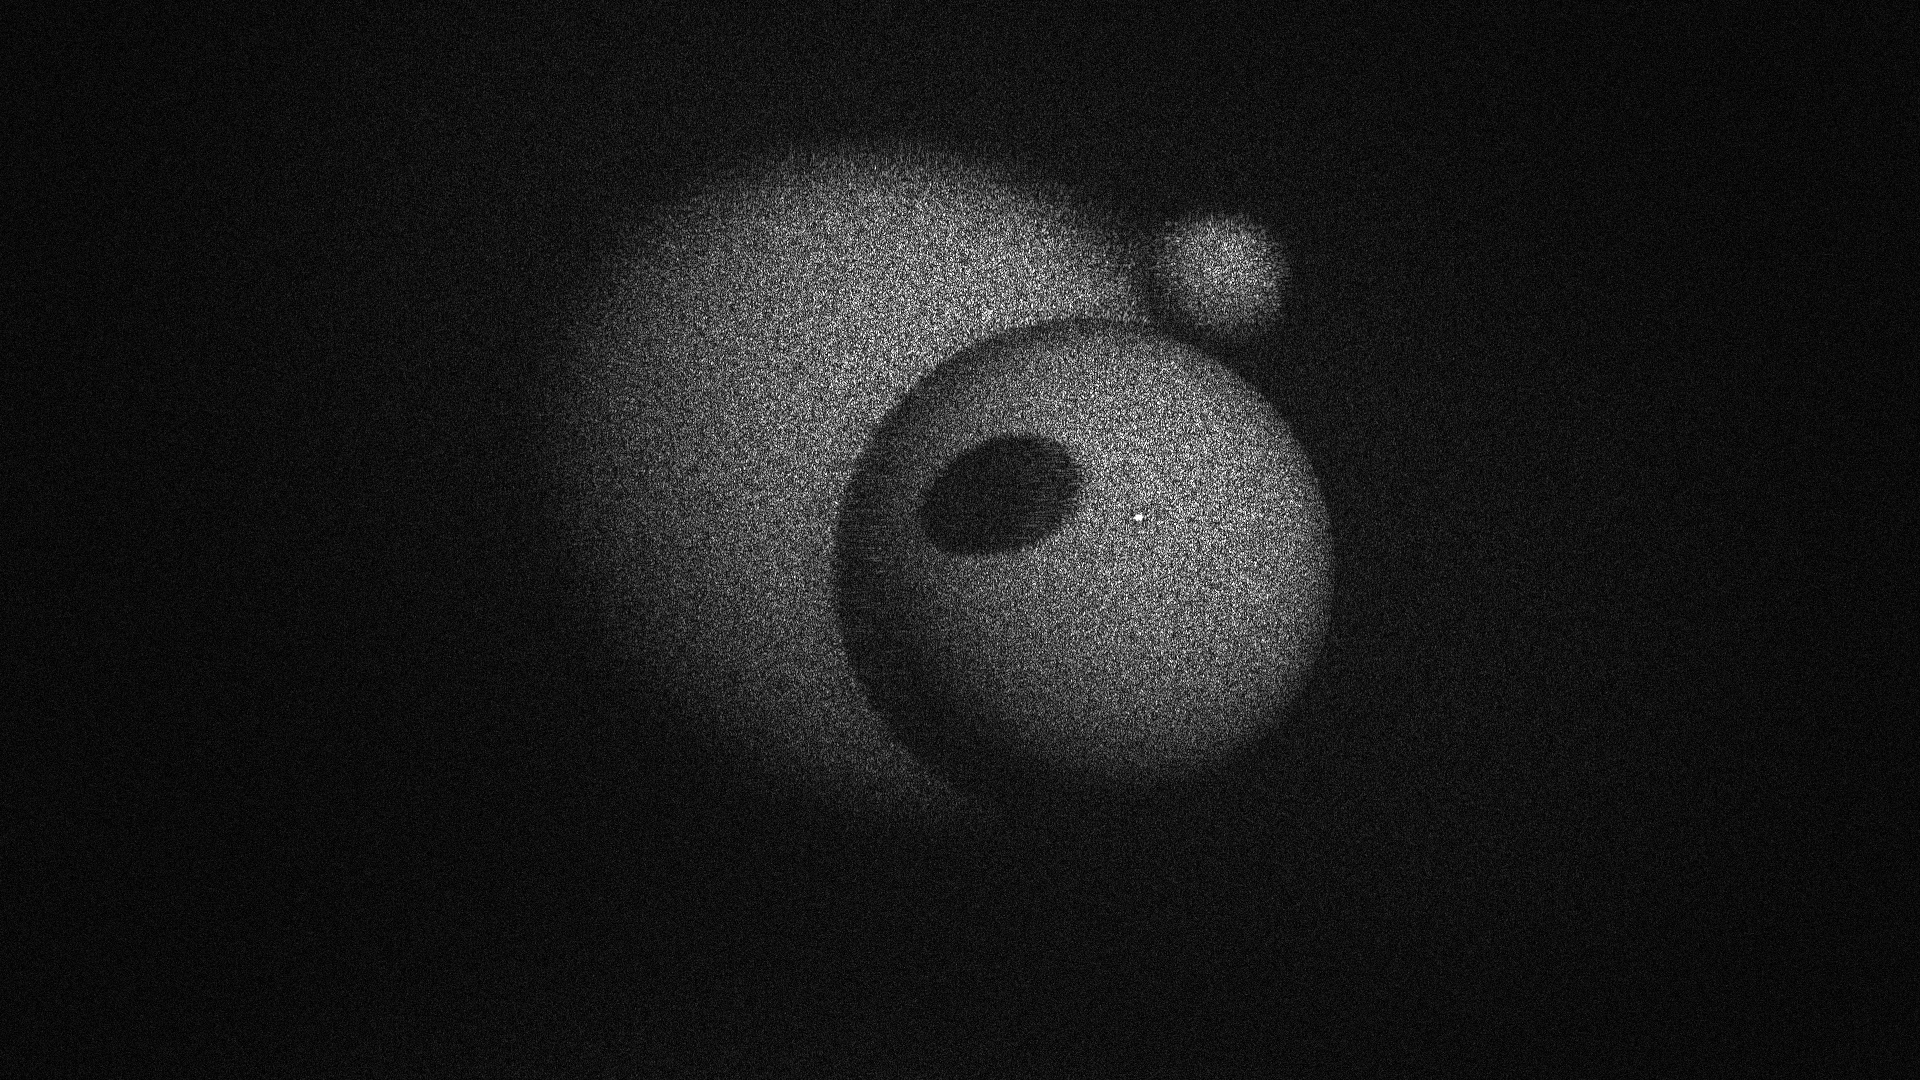
\includegraphics[width=1\textwidth]{simulated}
        \caption{Simulación}
        \label{fig:reconstruccion-simulacion}
    \end{subfigure}
    
    \begin{subfigure}{1\textwidth}
        \centering
        \includegraphics[width=1\textwidth]{reconstruction_lab}
        \caption{Propagación mediante un SLM}
        \label{fig:reconstruccion-laboratorio}
    \end{subfigure}
    \caption{Resultados de la reconstrucción de la escena tanto por simulación como en el laboratorio.}
    \label{fig:reconstruccion}
\end{figure}

\begin{figure}[H]
    \centering
    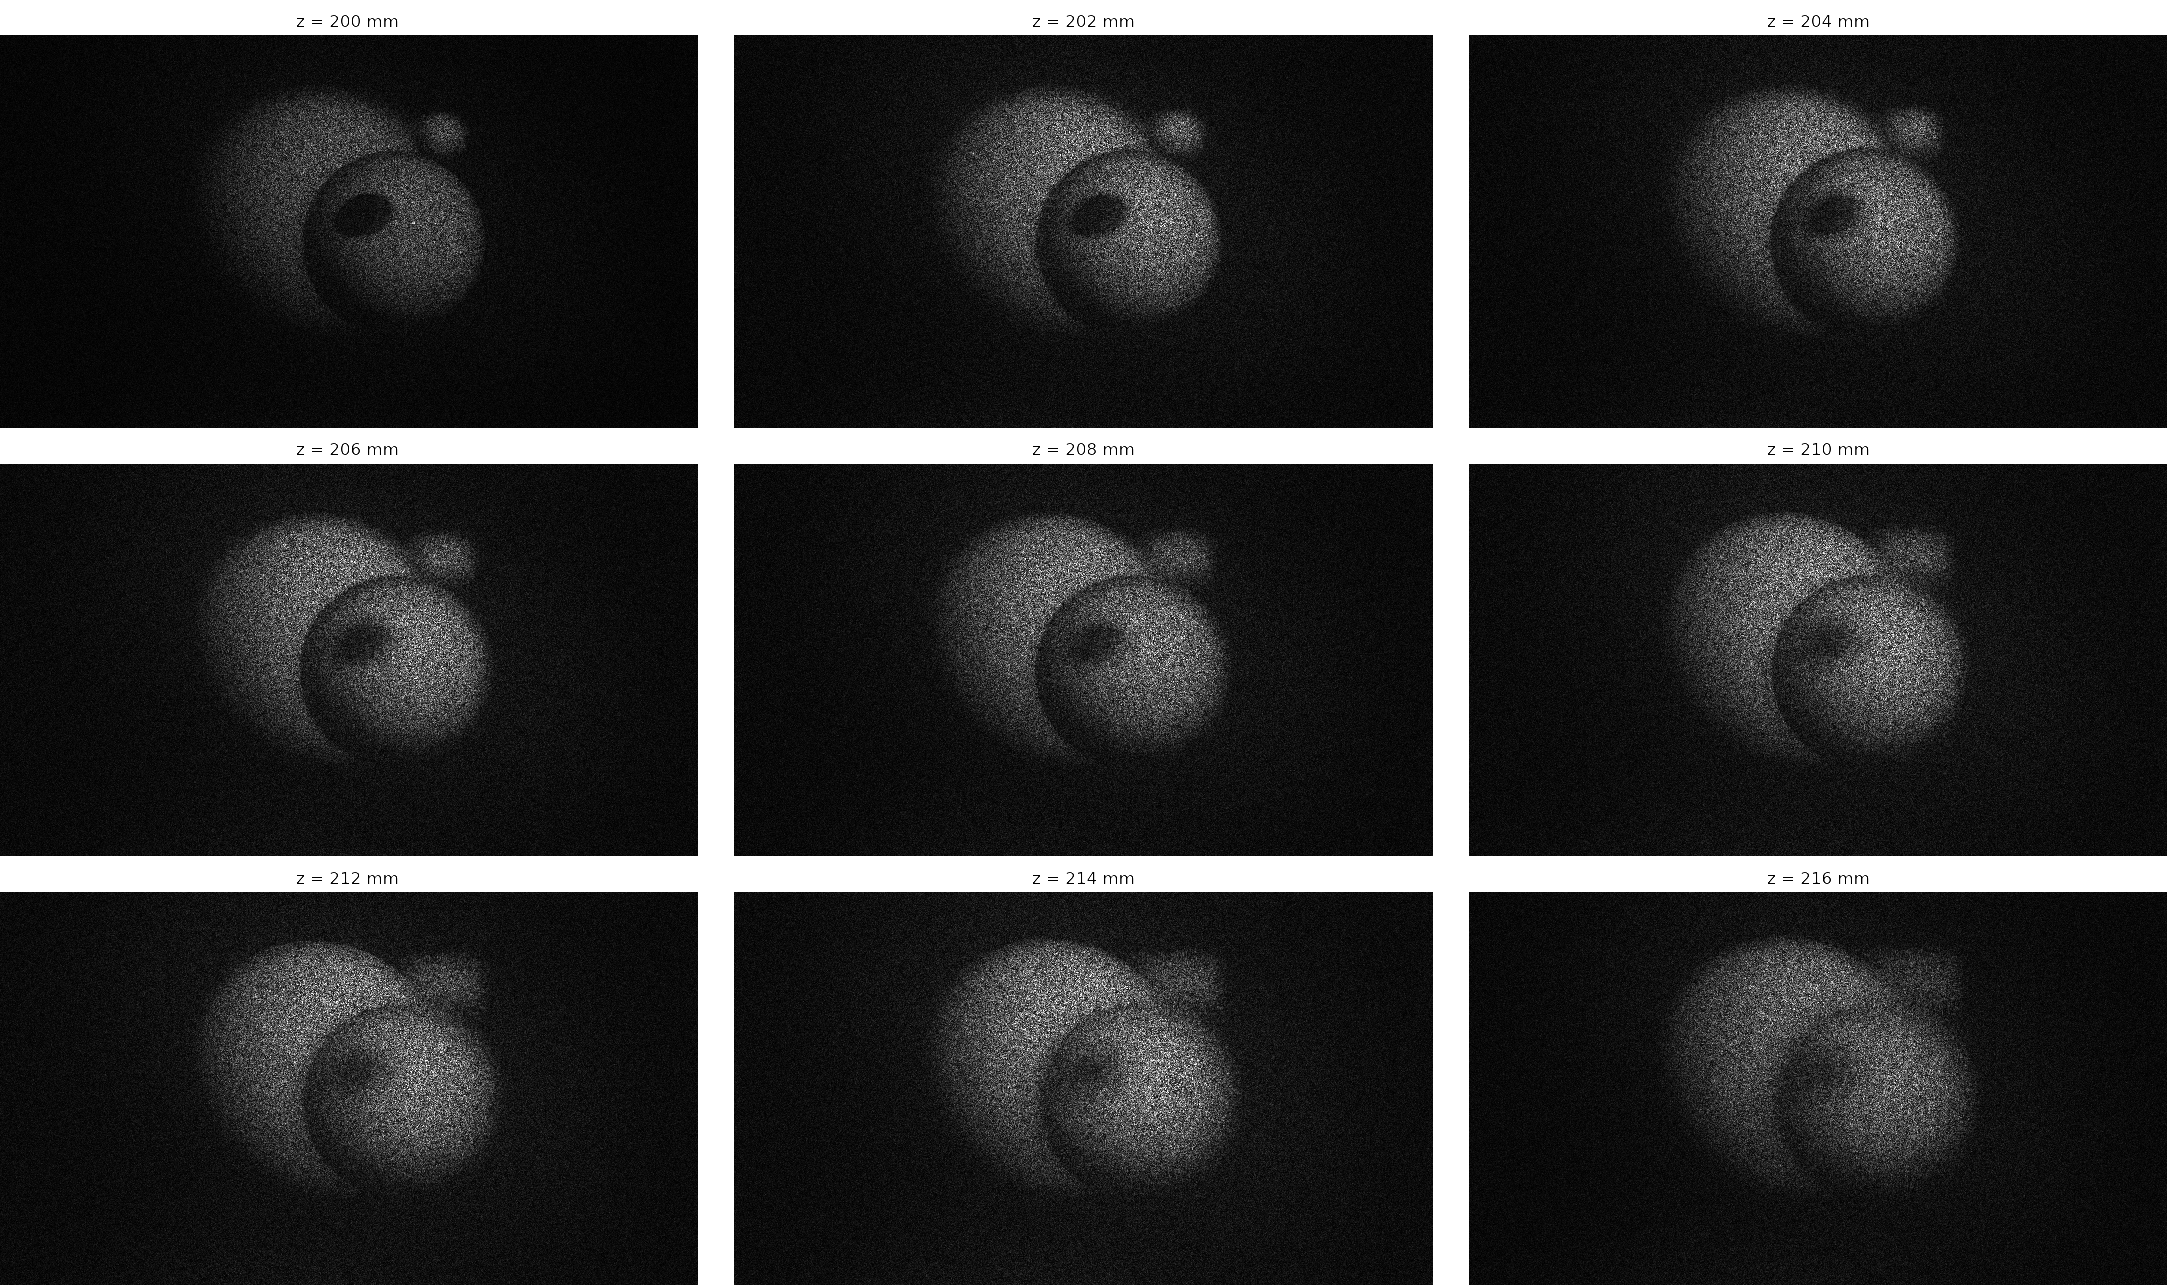
\includegraphics[width=1\textwidth]{reconstruction-figure}
    \caption{Simulación de la propagación para distintos valores de $z$.}
    \label{fig:reconstruccion-figura}
\end{figure}

\section{Técnicas de paralelización}

La computación paralela es un tipo de computación en la que muchos cálculos o procesos se pueden llevar a cabo simultáneamente \cite{Almasi:1989}. Existen varias técnicas de paralelización entre las que se encuentra la que se utilizará en este trabajo, el paralelismo de datos. Esta técnica consiste en dividir los datos entre distintos hilos de procesamiento. Por ejemplo, se podría dividir una imagen en píxeles, y operar a nivel de píxel o en bloques.

\subsection{CPU}

Las unidades centrales de procesamiento (CPUs) actuales cuentan con múltiples núcleos, lo que permite la ejecución paralela de múltiples hilos de procesamiento. Cada hilo puede ejecutar una serie de instrucciones de manera independiente, permitiendo la realización de tareas en paralelo.

Para aprovechar los diferentes núcleos de la CPU es necesario dividir el trabajo para diferentes hilos (o threads, en inglés). En el caso de un trazador de rayos, el método más sencillo de distribuir el trabajo es dividiendo la imagen en píxeles y asignando a cada hilo un rango de píxeles sobre los que operar. Este método cuenta con la limitación de que puede darse el caso de que un hilo acabe antes que otro. 

Para solucionar este problema se puede introducir el uso de un grupo de hilos (o thread pool, en inglés), al cuál se le puede asignar una serie de tareas que los hilos que lo forman ejecutan. Al dividir el trabajo en más tareas que hilos, se soluciona la limitación anterior. Se ha de tener en cuenta que la gestión de los hilos y las tareas tiene un coste computacional.

En el trazador de rayos implementado se ha dividido la imagen en líneas de píxeles y se ha optado por el uso de un grupo de hilos. La elección se debe principalmente a que el primer hilo suele terminar mucho antes que el último ya que en la mayoría de las escenas no se incluyen objetos en la parte superior. Esto no ocurre en el caso del trazador de rayos modificado para generar hologramas, ya que cada píxel lanza un rayo a cada punto y los hilos terminan con menor varianza. Por este motivo y por el coste extra del grupo de hilos, se ha optado por no utilizar grupos de hilos en la generación de hologramas.

\subsection{GPU}

Las unidades de procesamiento gráfico (GPUs) son componentes hardware diseñados originalmente para la renderización de gráficos. Sin embargo, debido a su arquitectura masivamente paralela, también son altamente eficaces en la realización de cálculos matemáticos complejos y tareas que pueden beneficiarse del paralelismo masivo.

Las GPUs están compuestas de miles de núcleos más simples y especializados que los de las CPUs. Esto permite la ejecución de miles de hilos simultáneamente, comparado con las CPUs que no suelen superar los 256 hilos.

Para poder utilizar una GPU, es necesario el uso de bibliotecas o herramientas especiales que faciliten la programación en GPUs, como CUDA, exclusivo de Nvidia, o OpenCL. Estas herramientas permiten escribir código el cual puede ser ejecutado en la GPU. En el caso de CUDA, el lenguaje es similar a C++. Por esto y porque la GPU de la que se dispone es Nvidia, se ha escogido CUDA para este trabajo \cite{Nvidia:2024}.


Como se ha mencionado anteriormente, el computo de un trazador de rayos puede ser dividido entre cada uno de los píxeles, lo que hace que las GPUs puedan acelerar significativamente el algoritmo. Cada píxel puede ser procesado por un núcleo diferente.

CUDA es una plataforma de computación paralela y una API creada por Nvidia que permite a los desarrolladores utilizar la GPU para tareas de computación general. Proporciona una extensión al lenguaje de programación C++ que incluye una serie de funciones y directivas para interactuar con la GPU. En CUDA, el código se divide en tres tipos. El tipo host (anfitrión) es el código que se ejecuta en la CPU. El tipo device (dispositivo) es el código que se ejecuta en la GPU. Y el tipo kernel es el código que se llama desde la CPU y asigna el trabajo a la GPU.

\subsection{Implementación}

La paralelización mediante hilos se ha implementado asignando un rango de lineas a cada hilo, las cuales se calculan y almacenan en memoria compartida. 

La paralelización mediante grupos de hilos se ha implementado gracias a la librería BS::thread\_pool. Al grupo se le añade numero de inicio, numero de fin, el numero de bloques en los que dividir el trabajo y una función que, dado un numero de linea, la calcula.

Por último, la paralelización en CUDA se ha implementado mediante un kernel. Una vez los datos necesarios están almacenados en memoria compartida o memoria de la GPU, se ejecuta un kernel en bloques suficientes para cubrir el tamaño de la imagen, en el que está definido como calcular un píxel. 


\section{Resultados}

\subsection{Tablas comparativas de tiempos.}

Para la obtención de los tiempos de este apartado se han utilizado dos ordenadores con las siguientes CPUs y GPUs: 

\begin{itemize}
    \item Ordenador 1:
    \begin{itemize}
        \item CPU: Intel i7 7700K (8 hilos, 4.4GHz)
        \item GPU: Nvidia RTX 3070 (5888 núcleos)
    \end{itemize}
    \item Ordenador 2:
    \begin{itemize}
        \item CPU: Intel i7 9900K (16 hilos, 4.7GHz)
        \item GPU: Nvidia RTX 2060 (1920 núcleos)
    \end{itemize}
\end{itemize}

Todos los tiempos se han obtenido al calcular la escena descrita anteriormente (\autoref{fig:holograma-cgi}) con un sensor de 1920 x 1080 píxeles. 

El primer resultado obtenido (\autoref{fig:grafico-cpu}) compara las dos CPUs con distintos números de puntos y el numero máximo de hilos menos uno. Se puede observar una correlación lineal entre tiempo y numero de puntos en las dos CPUs, esta correlación se utilizará en los siguientes resultados para obtener los datos en tiempos aceptables. Exceptuando el primer resultado de cada CPU (poca carga de trabajo), la media de la primera CPU es de 2.85 puntos por segundo, comparado con los 27.95 de la segunda (9.8 veces mas rápida). 

\begin{figure}[H]
    \centering
    \includegraphics[width=1\linewidth]{grafico_cpu}
    \caption{Por hacer: Caption y hacer la figura presentable}
    \label{fig:grafico-cpu}
\end{figure}

En la \autoref{fig:grafico-gpu} se comparan las dos GPUs de la misma manera. La media de la primera GPU es de 91.26 puntos por segundo y la de la segunda es de 50.14, siendo la primera 1.82 veces mas rápida respecto a la segunda y 3.27 veces respecto a la CPU más rápida.

\begin{figure}[H]
    \centering
    \includegraphics[width=1\linewidth]{grafico_gpu}
    \caption{Por hacer: Caption y hacer la figura presentable}
    \label{fig:grafico-gpu}
\end{figure}

Finalmente se han obtenido resultados para distintos números de hilos de las CPUs. Como se puede ver en la \autoref{fig:grafico-hilos}, el aumento del número de hilos conlleva a un aumento del rendimiento no lineal, esto puede deberse al coste de crear y gestionar hilos, la contención por recursos compartidos y el aumento de los fallos de caché y de los conflictos de acceso a la memoria.

\begin{figure}[H]
    \centering
    \includegraphics[width=1\linewidth]{grafico_hilos}
    \caption{Por hacer: Caption y hacer la figura presentable (solo 1 linea 2º CPU)}
    \label{fig:grafico-hilos}
\end{figure}

\underline{Por hacer: Recalcular 0.4M puntos}

\section{Conclusiones}

\section{Calendario}

\underline{Por hacer: detallar más}

\begin{itemize}
    \item Enero: Inicio proyecto, Implementación RTIOW, UI, Paralelización CPU.
    
    \item Febrero: Instalación del entorno CUDA, Migración del código C++ a CUDA, Añadir fuente de luz puntual, Añadir soporte de triángulos y OBJ, BVH para CPU.
    
    \item Marzo: Añadir CGH, paralelización CPU.

    \item Mayo: Propagación, CGH en CUDA.

    \item Junio: Limpieza del código, Memoria.

    \item Julio: Memoria.
    
\end{itemize}

\section{Trabajo futuro}

\section{Dificultades encontradas}

Durante la realización de este trabajo se han encontrado distintas dificultades descritas a continuación, clasificadas como normales, medias, difíciles y muy difíciles.

La primera dificultad encontrada ha sido el uso de un sistema para gestionar el proyecto (difícil), ya que el estándar de C++ no incluye uno. Se ha utilizado CMake ya que es el más popular, permite añadir librerías y soporta el uso de CUDA. Aún utilizando CMake, es necesario conocer varios argumentos de los distintos compiladores (clang para C++ y nvcc para CUDA) para conseguir que funcione correctamente. 

La principal dificultades relacionada con CUDA es la gestión de memoria (difícil). Versiones modernas de CUDA soportan memoria gestionada automáticamente, lo cuál simplificaría el problema si no fuera porque se hace uso de características no soportadas, como el polimorfismo para materiales y objetos de la escena. Por ello se ha tenido que gestionar la memoria manualmente. 

Otra dificultad relacionada con CUDA es la depuración (difícil). Las herramientas de depuración para GPUs no son tan maduras como las de CPUs y esto hace que sea complicado encontrar errores que no ocurren al ejecutar el programa en CPU. 

La librería estándar de C++ para CUDA no incluye algunas funcionalidades (normal) como pueden ser vectores (std::vector) y números complejos (std::complex). La solución para el primer caso es hacer uso de matrices y, para el segundo, utilizar otra opción ofrecida en CUDA (thrust::complex).

CGH: depuración, triángulos

\printbibliography[heading=bibintoc]

\section{Anexos}

\subsection{Licencias}

\subsection{Repositorios}

\end{document}
